% 
% Annual Cognitive Science Conference
% Sample LaTeX Paper -- Proceedings Format
% 

% Original : Ashwin Ram (ashwin@cc.gatech.edu)       04/01/1994
% Modified : Johanna Moore (jmoore@cs.pitt.edu)      03/17/1995
% Modified : David Noelle (noelle@ucsd.edu)          03/15/1996
% Modified : Pat Langley (langley@cs.stanford.edu)   01/26/1997
% Latex2e corrections by Ramin Charles Nakisa        01/28/1997 
% Modified : Tina Eliassi-Rad (eliassi@cs.wisc.edu)  01/31/1998
% Modified : Trisha Yannuzzi (trisha@ircs.upenn.edu) 12/28/1999 (in process)
% Modified : Mary Ellen Foster (M.E.Foster@ed.ac.uk) 12/11/2000
% Modified : Ken Forbus                              01/23/2004
% Modified : Eli M. Silk (esilk@pitt.edu)            05/24/2005
% Modified : Niels Taatgen (taatgen@cmu.edu)         10/24/2006
% Modified : David Noelle (dnoelle@ucmerced.edu)     11/19/2014

%% Change "letterpaper" in the following line to "a4paper" if you must.

\documentclass[10pt,letterpaper]{article}

\usepackage{cogsci}
\usepackage{pslatex}
\usepackage[natbibapa]{apacite}
\usepackage{amsmath}
\usepackage{amssymb}
\usepackage{xcolor}  % for \todo
\usepackage{graphicx}
\usepackage{csquotes}
\MakeOuterQuote{"}
\usepackage{booktabs}

\title{Compositional sub-goal representations for planning and problem-solving}

\newcommand{\todo}[1]{\textcolor{red}{\textsc{[TODO: #1]}}}
\newcommand{\red}[1]{\textcolor{red}{#1}}
\newcommand{\MISSING}{\red{XX}}

\author{TODO}


\begin{document}

\maketitle


\begin{abstract}
When faced with a large and complex problem, people naturally break it up into several smaller and simpler problems. This hierarchical decomposition of an ultimate goal into sub-goals facilitates planning by reducing the number of factors that must be considered at one time. However, it can also lead to suboptimal decision-making, missing opportunities to make progress towards multiple subgoals with a single action. This potential for suboptimality can be ameliorated by considering multiple subgoals at once, but at the cost of increasing the number of factors that must be considered and thus increasing the computational burden of planning. Here, we present a model of planning with compositional goal representations and show that it explains the errors people make in a Towers of London task better than a limited-depth search model. Our results suggest that people are capable of representing and pursuing multiple subgoals at once, but that the number of subgoals is generally quite limited. Furthermore, we find that the degree to which composite goal representation is limited may be an important latent dimension for explaining individual differences in planning ability. Finally, we (hopefully!) find that the inferred representational limitations are sensitive to the cost of suboptimal planning, indicating that people may rationally choose a goal representation that trades off between representational costs and decision quality.

\textbf{Keywords:} 
planning; hierarchy; goals
\end{abstract}


\section{Introduction}

It's Tuesday afternoon and you have a list of errands to run before you can return home to watch last night's episode of \textit{The Bachelor}. You need to mail a letter, pick up broccoli for tonight's stir fry, and drop off a book at the library. You are eager to get home to see whether Hannah B. received one of the coveted roses, and thus want to accomplish these tasks as expediently as possible. There are two library locations, four grocery stores, and who knows how many mail boxes in your town; how do you decide which location of each to visit, and in what order? Unfortunately, you have been presented with the generalized traveling salesman problem, which is known to be NP-hard (that is, potentially very difficult to solve). You might simplify the problem by focusing on only one errand at a time, completing it as quickly as possible from wherever the last errand left you. But by ignoring your other tasks when planning how to complete one, you might miss the opportunity to save time by going to the library location that is further from your house, but right next to a grocery store.

% To solve complex problems, it is necessary to break them down into subproblems [cite AI]. People do this []. The standard model of organizing problems into subproblems 

% The ability of people to solve problems such as these has typically been formulated in terms of search \citep{NewellSimon1972}. Under this theory, people construct a "decision tree" that represents possible courses of actions and their outcomes, searching over the tree for the best possible plan. However, these decision trees can quickly become too large to search exhaustively, necessitating approximation strategies \citep{Huys2015}. A particularly valuable strategy for directing search is \textit{subgoaling} \citep{Donnarumma2016}. By focusing on one subgoal at a time, one can ignore irrelevant actions and features of the environment, effectively reducing the size of the decision tree to search over \citep{Dietterich2000}. However, by dividing the space in this way, one will miss opportunities to make progress towards multiple subgoals at once. Of course, people often \textit{do} identify these opportunities, posing a problem for the standard one-at-a-time model of subgoal pursuit.

The ability of people to solve problems such as these has typically been formulated in terms of search \citep{NewellSimon1972}. Under this theory, people form a plan of action by searching over an internal representation of the problem. However, the combinatorial explosion of possible sequences of actions makes exhaustive search intractable in all but the simplest cases. This necessitates approximation strategies \citep{Huys2015}. A particularly valuable strategy for directing search is \textit{subgoaling} \citep{Donnarumma2016}. By focusing on one subgoal at a time, one can ignore irrelevant actions and features of the environment, effectively reducing the dimensionality of the problem space \citep{Dietterich2000}. However, this reduction comes at a cost. Standard goal-setting models assume that subgoals are \textit{context-free} in the sense that they are pursued independently, without consideration of the ultimate goal or future subgoals. As a result, opportunities to make progress towards multiple subgoals at once will be missed. Nevertheless, people often \textit{do} identify these opportunities, posing a problem for the standard one-at-a-time model of subgoal pursuit.

How can we reconcile the strong evidence for the role of goals in structuring human behavior \citep{Cooper2006} with the apparent ability of people to "kill two birds with one stone?" One possibility is that, contrary to the standard model, people are not limited to pursuing one goal at a time. That is, perhaps they choose a \textit{subset} of goals, and construct a plan that is optimal with respect to that subset.
They might ask themselves, for example, "what is the fastest way to get to both a grocery store and a library?", leaving future goals such as dropping off a letter for future consideration.
We formalize this theory in a hierarchical planning framework.
At the abstract level, the agent dynamically constructs composite goals (or \textit{multigoals}) from a set of primitive goals. Then, at the concrete level, the agent searches for a plan that achieves the composite goal, disregarding any other potential future goals. To test the model, we first identify a classic task from the problem solving literature that can provide a behavioral signature of the subgoal representations underlying our participant's choices (if such representations exist). Using a Bayesian modeling framework, we can dissociate constraints on the number of subgoals they can pursue at once from goal-agnostic constraints on the depth of search. Finally, we use formal model comparison to demonstrate that the multigoal model explains participant behavior better than both goal-free and single-goal models.

We begin the paper by discussing relevant theoretical approaches to planning and problem solving. We then present a formal model of planning with composite \textit{multigoals}. Next, we present an experiment designed to dissociate the predictions of the multigoal model from those of standard depth-limited search and hierarchical planning models. We discuss the application of the general model to the specific problem, and present model fitting results. We conclude with a discussion of \todo{pull from discussion}.

\section{Background}
Much previous work in psychology has studied the strategies people use to make planning and problem solving tractable. In particular, we focus on two non-exclusive classes of strategies that have been studied: \textit{tree search} and \textit{hierarchical decomposition}. Tree search strategies take inspiration from algorithms based on search through a decision tree, in which possible plans are simulated forward and evaluated~\citep{}. For example, rather than consider plans that are arbitrarily long, people can engage in \textit{depth-limited search} that focuses resources on plans that can be taken within a certain time horizon~\citep{MacGregor2001,Keramati2016,Krusche2018}. Alternatively, they may rely on heuristics to guide search~\cite[chap. 5]{Anderson1990} or use local signals of progress to avoid less promising plans without explicitly considering them~\citep{Huys2012}.

However, approaches such as depth-limited search and heuristics are, in a sense, limited by their locality---what if the goal is many timesteps away, or even just out of reach? What if the heuristic cues are uninformative or simply do not exist? This, in part, motivates complementary approaches based on \textit{hierarchical decomposition}, in which a problem is holistically broken into sub-problems, each of which are then solved in the right order~\citep{sacerdoti1974planning, botvinick2012hierarchical}. Such an approach can make decision-making easier by reducing the resources needed to solve a given sub-problem at a particular time~\citep{VanDijk2011, Maisto2015}. But this raises yet another problem: What is a good way to break down a task? And what if the particular decomposition could be improved?

The Sussman anomaly exemplifies what happens when a decompositions are too brittle (Figure~\ref{}, \citeNP{}). In the Sussman anomaly, an agent plans with respect to a single subgoal at a time (e.g., put block A on top of block B) without considering the larger context of that subgoal with respect to other subgoals. That is, subgoals are completely \textit{context-free}. This can lead to inefficiencies (e.g., having to move A and B again in order to get B on top of C) that could have been avoided. More generally, some efficiencies in problems can only reliably be achieved by planning with respect to multiple subgoals as plans based on individual subgoals may be myopic, greedily optimizing for the subgoal at hand. For instance, Figure 1 demonstrates a case where considering a single subgoal might result in a suboptimal solution that is avoided when considering multiple subgoals. More generally, agents planning with respect to different numbers of subgoals take actions with different probabilities in various states, which forms the basis of our modeling framework.

% \subsection{Search and its limitations}

% Many of the hallmarks of higher level human cognition, such as problem solving \citep{NewellSimon1972}, strategic reasoning \citep{Holding1985}, and planning \citep{Simon2011} have been modeled as search over a decision tree. In each case, the problem at hand is represented as a tree, with nodes representing possible future states and branches representing decisions one could make in those states.

% In complex domains, exhaustive search is computationally intractable; thus search must be curtailed in some way. When extensive experience is available, people may avoid search by relying on model-free reinforcement learning \citep{Keramati2011,Kool2017} or cached action sequences \citep{Huys2015}. When rewards are dense, they may use these local signals of progress to avoid less promising branches of a decision tree \citep{Huys2012}. However, many of the problems people encounter in their daily lives lack such structure.

% When full search is infeasible and progress cues are limited or unreliable, people may have to impose arbitrary constraints on their search. The simplest such constraint is to put a limit on how far into the future you look. So-called \textit{depth-limited search} has been incorporated into several models of human search \citep{MacGregor2001,Keramati2016,Krusche2018}.
% Under this strategy, the searcher considers all possible action sequences of some length $d$, and chooses the one that gives the best intermediate outcome. How the intermediate outcome is defined depends on the problem domain, and can have substantial effects on the choices that are ultimately made. For planning in reward-maximization problems, this outcome is typically the sum of rewards one receives along this path (perhaps augmented with a learned value of the final state; \citealp{Keramati2016}). In problem solving settings, there are typically no intermediate rewards, and a heuristic estimate of distance to the goal state is used to evaluate partial plans \cite[chap. 5]{Anderson1990}. A good heuristic can reduce or even eliminate the need to look far into the future, resulting in a "hill climbing" strategy. But for more challenging problems, people may require more complex strategies to guide their search.

% \subsection{Subgoals and hierarchical planning}
% Many of the complex problems that people face in their daily lives can naturally be decomposed into smaller problems. People can take advantage of this structure by setting \textit{subgoals}, intermediate goals (e.g. pick up broccoli) that each contribute to achieving a larger goal (cook dinner) which itself may be part of an even broader goal (avoid starvation). This approach can ultimately make decision-making easier, reducing working memory requirements \citep{VanDijk2011} and/or computational complexity \citep{Maisto2015}. However, it also creates a new problem: How should one choose subgoals that will both accomplish the ultimate goal, and also be relatively easy to solve individually? \textit{Hierarchical planning} is one way to answer this question. 

% In hierarchical planning, search occurs at different levels of abstraction~\citep{sacerdoti1974planning}. At the top level, one plans over potential sequences of subgoals to pursue in order to accomplish the ultimate goal. Each subgoal then becomes its own planning problem in which one plans over sequences of actions (or perhaps simpler subgoals) to accomplish that subgoal. Hierarchical planning has been studied as a way in which humans learn to solve complex tasks~\citep{botvinick2012hierarchical} and also as a method for scaling up automated planning systems~\citep{kaelbling2010hierarchical}. Research on hierarchical planning has traditionally focused on learning or planning given a particular decomposition~\citep{sacerdoti1974planning, parr1998reinforcement}, and more recent approaches have examined learning hierarchical planning representations through interaction with an environment or from another agent's demonstrations~\citep{bacon2017option, cobo2014abstraction}. From a functional perspective, hierarchical task decompositions enable adaptive systems to trade off behavioral optimality with computational resources. A key question is then what properties of a decomposition facilitate this tradeoff.

% Algorithms for learning policies in hierarchically structured tasks assume that subpolicies are insensitive to the context they're executed in. The assumption that subpolicies are context-free is termed \textit{recursive optimality} \citep{Dietterich2000} and ensures that these subpolicies can flexibly be applied in many contexts. The Sussman anomaly exemplifies a case where acting optimally with respect to individual subgoals renders a problem impossible to complete. This issue can be avoided by changing the structure of subgoals or planning with respect to multiple subgoals. More generally, some efficiencies in problems can only reliably be achieved by planning with respect to multiple subgoals as plans based on individual subgoals may be myopic, greedily optimizing for the subgoal at hand. For instance, Figure 1 demonstrates a case where considering a single subgoal might result in a suboptimal solution that is avoided when considering multiple subgoals. More generally, agents planning with respect to different numbers of subgoals take actions with different probabilities in various states, which forms the basis of our modeling framework.

% \todo{This might be too much detail for the background}
% Our work here can be understood as analyzing \textit{subgoal resolution} as a factor in the construction of hierarchical plans in humans. At a particular moment in time, a person will have a subgoal they want to complete. Compare the subgoal ``mail a letter'' with the subgoal ``mail a letter AND go to the grocery''. The second subgoal has higher \textit{resolution} than the first in that it is more specific and picks out a strictly smaller set of states as acceptable for completion. This factor is a key element for any hierarchical planning scheme. For example, in formalisms such as the options framework~\citep{sutton1999between}, macro-actions (i.e., options) are defined in part by the set of states in which one exits an option. Our approach can be understood then as considering the complexity of the predicates defining a termination condition when people hierarchically decompose a task.

\begin{figure*}[ht]
    \centering
    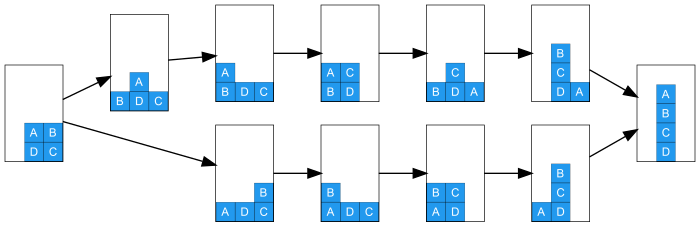
\includegraphics[width=0.9\textwidth]{example-4-block.png}
    \caption{Planning to stack C on D might result in either of the two depicted plans, where A or B is first removed. Removing A first (the lower plan) winds up being more efficient, taking 1 step fewer to achieve the goal state. When planning with respect to two subgoals (stack C on D and stack B on C), an agent will always choose to remove A first (like in the lower plan) since they are optimizing for the eventual placement of B. Blocks are green when their corresponding subgoal has been satisfied.}
\end{figure*}



\section{Planning with multigoals}
\newcommand{\multigoal}{\mathcal{G}}

Multigoals extend a standard goal-based hierarchical planning algorithm by allowing for new subgoals to be constructed on the fly by composing existing, primitive subgoals. Formally, we define a multigoal,  $\multigoal$, as a set of primitive subgoals. Following the options framework \citep{sutton1999between}, a subgoal $g$ is defined by a function 
$\beta_g: \mathcal{S} \rightarrow \{0, 1\}$
that indicates whether a state satisfies the given subgoal. A multigoal is satisfied by a state that satisfies all of its component subgoals; thus, a multigoal's satisfaction function is defined
$\beta_{\multigoal}(s) = \prod_{g \in \multigoal} \beta_g(s)$. Although multigoals can be integrated into arbitrarily deep hierarchical planning models for stochastic environments, we focus on the simplest case of a two-level hierarchy and deterministic environments. At the abstract level the agent chooses a multigoal based on the current state and ultimate goal. At the concrete level, the agent attempts to find a sequence of actions that satisfies the current multigoal.

A full abstract-level planning model would both identify possible subgoals and also choose which ones to pursue at each step. However, to simplify the problem, we assume that the goals and their ordering are given. That is, the agent receives an ordered set of subgoals $\{ g_1, g_2, \dots g_n  \}$ such that completing all $n$ subgoals in order amounts to solving the ultimate goal. The abstract-level phase of planning is thus reduced to selecting a number of subgoals to pursue; we call this number $k$. Given a selection of $k$ and the multigoal in a given state, $\multigoal(s; k)$ is simply the set of the next $k$ incomplete subgoals. For example, if $g_1$ has been completed ($\beta_{g_1}(s) = 1)$ and $k=2$, we would have $\multigoal(s; k=2) = \{ g_2, g_3 \}$. \red{Admittedly, this simplifying assumption eliminates a considerable amount of interesting complexity. However, it allows us to look for experimental evidence for multigoals without tackling the full problem of multigoal selection. Relaxing this assumption is an important direction for future work.}

% \begin{equation}
%   \multigoal(s; k) = \{g_i \dots g_{i+k-1} \} \text{ s.t. } 
%     \beta_{g_{i-1}}(s) = 1 \wedge \beta_{g_i}(s) = 0
% \end{equation}

Given a multigoal $\multigoal$, concrete-level planning uses tree search to find a lowest-cost path $\pi$ that satisfy all subgoals in $\multigoal$. This search process may be depth-limited. If no path of length $d$ or less can be found that satisfies all the subgoals, the model chooses a path that satisfies the largest possible number of subgoals. Thus, the action sequence is chosen by
%
\begin{equation}\label{eq:concrete}
  \arg\max_\pi 
    \sum_{g \in \multigoal} \beta_g(s_\pi) - \lambda |\pi |
    \; \text{ s.t.  } |\pi| \leq d,
\end{equation}
%
where $s_\pi$ is the final state on the path defined by the action sequence $\pi$ and $\lambda$ is a very small positive constant, with the effect that $\pi$ is chosen to maximize the first term (number of subgoals completed), using the second term (path length) as a tie-breaker.

There are several special cases of the model worth highlighting. When $k = 1$, we recover a standard hierarchical planning algorithm in which only one subgoal is pursued at a time. When $k = \infty$, we recover a standard depth-limited search model with a heuristic cost function defined by the number of incomplete subgoals. When $d = \infty$, the model optimally achieves each multigoal, but may still perform suboptimally because future subgoals are not considered. And when $d = k = \infty$, the model always makes optimal choices.


\section{Experiment 1: Measuring human multigoaling}

To test the predictions of the multigoal model, we conducted a Tower of London (ToL) experiment \cite{Shallice1982}. The classic ToL task is based on the Tower of Hanoi problem, removing the constraints imposed by different-sized disks, but adding a limit to how many disks can be on each peg. Our variant of ToL uses blocks instead of disks and removes the restrictions on stack height. We additionally mark the blocks with letters and use a single standard goal position to reduce working memory requirements. This results in an unambiguous subgoal ordering \citep{Kaller2011}: One must put blocks in their place in reverse alphabetical order.
% Thus, the model's simplifying assumption that the order of subgoals is given is innocuous in this specific setting. 

% With these modifications to the rules, our experimental task resembles Blocks World, a domain used to investigate problem solving in artificial intelligence research \todo{XXX connect to Sussman}.

% \todo{Integrate the text below with the text above, probably cutting some extraneous material}

% Prior work \citep{Simon1975} has established various strategies people might use when solving ToH puzzles, and other studies have even taught specific strategies to people to examine the relationship between the underlying cognitive mechanisms implicated by these strategies and measures like response time \citep{Anderson2001} and fMRI signal \citep{Anderson2005}.


\subsection{Methods}
\subsubsection{Stimuli and procedure}

In each trial, participants are presented with two configurations of stacked blocks marked with letters of the alphabet and asked to rearrange the blocks in one stack to match the blocks in the other or goal stack (Fig. 2). Only the top block of a stack can be moved, and the board is limited to contain at most three spaces (columns) for stacks. In all trials, the goal stack contains the same blocks arranged in alphabetical order in the middle space. 

Participants completed three tutorial trials of increasing difficulty (a 3-block trial, a 4-block trial, and a 5-block trial) and then completed sixteen 6-block trials. Only the 6-block trials are analyzed below. Problems were selected to maximize the difference in likelihood of the fixed-$k$multigoal model (Equation~\ref{eq:likelihood-fixed}) and the limited depth model on data simulated from multigoal agents with $k \in \{ 1,2,3,4 \}$.

\begin{figure}[ht]
    \centering
    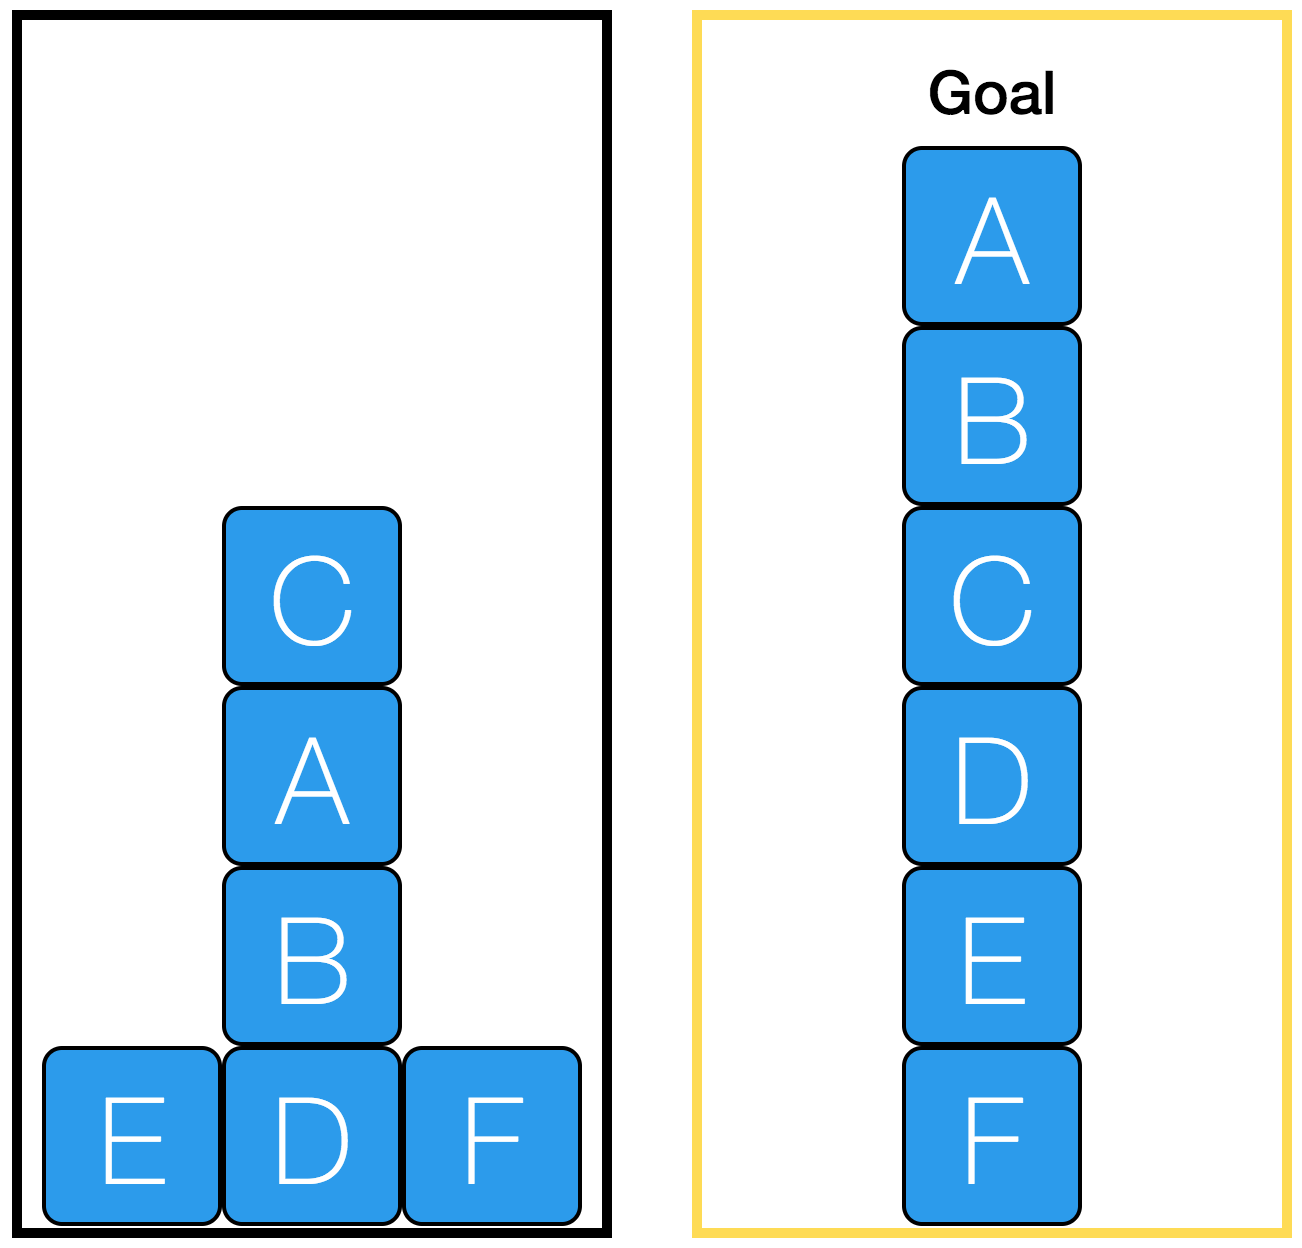
\includegraphics[width=6cm]{example-block-world.png}
    \caption{Experimental interface. On the left is the initial state which must be rearranged to match the goal state at right.}
\end{figure}

\subsubsection{Participants}
We recruited 41 participants from Amazon Mechanical Turk. Each participant received \$2 for completing the task, which took an average of 9 minutes.

\subsection{Model}
 
According to the proposed multigoal model, people can select multiple subgoals to pursue concurrently, attempting to create a plan that satisfies all $k$ subgoals in the fewest steps. In the experimental task, we define a subgoal as putting a block in its correct final position. Thus, we have an ordered set of subgoals $\{ g_F, g_E, g_D, g_C, g_B, g_A \}$ such that completing them in order necessarily solves the full problem. This satisfies the simplifying assumption required by the model, and \red{it is not unreasonable to assume that such a subgoal structure is apparent to the experimental participants.}


\newcommand{\A}{\mathcal{A}}
\newcommand{\U}{\mathcal{U}}

We now derive a likelihood to use for model fitting and comparison. Given a state and a value for $k$, the model selects a multigoal $\multigoal(s; k)$ which is the set of the next $k$ uncompleted subgoals. Then, given this multigoal and a value for $d$, we find a set of optimal paths given by Equation~\ref{eq:concrete}. In the case of ties, it is not obvious how to determine which path should be chosen because the probability of finding a given path depends on the specific search algorithm one uses, a detail we remain agnostic about. Thus the model simply divides probability uniformly among the set of unique first actions in any of the identified paths. Call this set $\A^*(s; k, d)$, which is a subset of all allowable actions $\A(s)$. We can now define the likelihood of taking a single action in a given state as
%
\begin{equation}\label{eq:likelihood-fixed}
  \Pr(a \mid s; k, d, \epsilon) = 
  (1 - \epsilon) \cdot \U(a \mid \A^*(s; k, d)) + 
  \epsilon \cdot \U(a \mid \A(s)),
\end{equation}
%
where $\U$ is the Uniform distribution. Note that by defining the likelihood for each action independently, we implicitly assume that participants re-plan at every step. Relaxing this assumption complicates model-fitting considerably, but it is an important direction for future work.

To test the multigoal model, in particular to evaluate whether people show evidence of pursuing more than one goal at a time, we employ formal model comparison. The comparisons of greatest interest are special cases of the full model. A standard depth-limited search model sets $k=\infty$ and has $d$ (the search depth) as a free parameter. A standard hierarchical planning or subgoaling model sets $k=1$, allowing for only one subgoal to be pursued at a time, and also has $d$ as a free parameter. In the full model, both $k$ and $d$ are free.

We consider two hypotheses for how $k$ and $d$ are chosen when they are free parameters. The first hypothesis is that the parameter is fixed for each individual. For example, one person might always consider two subgoals at a time ($k=2$)  and search fourteen steps into the future ($d=14$). The second hypothesis is that $k$ and $d$ vary from decision to decision, but follow some distribution that is particular to each individual. For example, one person might typically consider one subgoal at a time but occasionally pursue two (or rarely, three) subgoals at a time. We consider \red{two possible distributions for both $k$ and $d$}: the Geometric distribution and the Poisson distribution. Because these distribution both have a single parameter, introducing distributions over $k$ and $d$ does not increase the number of parameters in the model. To compute the likelihood, we integrate out the latent $k$ and $d$ parameters, which requires enumerating each parameter up to the value at which it results in optimal decision making (all greater values give the same prediction of optimal choices). Thus, for the models that put distributions over $k$ and/or $d$ with parameters $\theta_k$ and $\theta_d$ we have
%
% \begin{equation}\label{likelihood-dist}
% \begin{aligned}
%   \Pr(a \mid s; \theta_k, \theta_d, \epsilon) = 
%     \sum_{d=1}^{d^*}\sum_{k=1}^{k^*} 
%       \Pr(a \mid s; k, d, \epsilon) \Pr(k ; \theta_k) \Pr(d ; \theta_d) \\
%       + \Pr(a | s; k=\intfy, d=\infty, \epsilon)
%         \Pr(K > k^*; \theta_k) \Pr(D > d^*; \theta_d)
% .
% \end{aligned}
% \end{equation}
%
\begin{equation}\label{eq:likelihood-dist}
  \Pr(a \mid s; \theta_k, \theta_d, \epsilon) = 
    \sum_d \sum_k
      \Pr(a \mid s; k, d, \epsilon) \Pr(k ; \theta_k) \Pr(d ; \theta_d) \\
.
\end{equation}

We fit all models by maxmimum likelihood estimation. For discrete parameters we used grid search, considering all possible values of $k \in \{ 1 \dots 6 \}$ and values of $d \in \{1 \dots \MISSING \}$. For continuous parameters, we used \red{some convex optimizer} with \MISSING random initializations to mitigate the risk of finding local minima.


\subsection{Results}

\begin{figure}[t!]
    \centering
    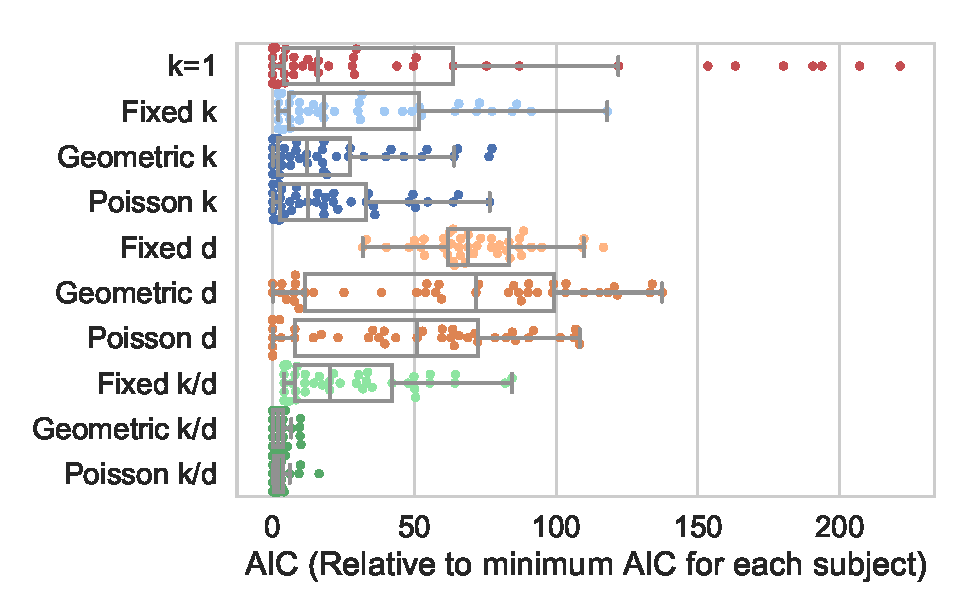
\includegraphics[scale=0.5]{model-fits}
    \caption{AIC for model fits. Each point is the model fit across all actions in all problems solved by a single participant.}
\end{figure}

\begin{table}[t!]
\centering
\begin{tabular}{lrrrr}
\toprule
Model         & \# Parameters & AIC   & LL    & \# Best fit \\
\midrule
Geometric k/d & 3 & \textbf{10533} & -5143 & 12 \\
Poisson k/d & 3 & 10541 & -5147 & 10 \\
Poisson k & 2 & 11234 & -5535 & 2 \\
Geometric k & 2 & 11250 & -5543 & 2 \\
Fixed k/d & 3 & 11518 & -5636 & 0 \\
Fixed k & 2 & 11705 & -5770 & 0 \\
Poisson d & 2 & 12364 & -6100 & 7 \\
k=1 & 1 & 12482 & -6200 & 6 \\
Geometric d & 2 & 13062 & -6449 & 2 \\
Fixed d & 2 & 13348 & -6592 & 0 \\
\bottomrule
\end{tabular}
\caption{Model comparison: Columns are number of parameters per participant, Akaike information criterion, log likelihood, and the number of participants best fit by the model.}
%, and Number of Participants best fit by the model (with parameters optimized separately)
\end{table}

 
Models were fit for each participant, see Figure 3.

Models with distributions over model parameters $k$ and $d$ were generally better fits than those with fixed parameters, suggesting that people flexibly adapt these limitations on planning.

Models with distributions over $k$ were better fits than models with distributions over $d$ in 28 out of 41 participants, suggesting that goal-based planning may better explain participant actions than depth limits in this task.

Of particular note is that many participants are best explained by a $k=1$ model or Geometric distribution with large $p$ (which acts like the $k=1$ model with probability $p$). The case of $k=1$ amounts to simple hierarchical planning, where search finds optimal paths towards the next incomplete subgoal. It's particularly interesting that the $k=1$ is a comparable fit to the best depth model in 27 out of 41 participants, suggesting that in at least this task even very simple goal representations are a strong constraint on search that can explain action comparably to well-established models of search.

The joint model with Geometric distributions over $k$ and $d$ is the best fit for 22 out of 41 participants and best overall fit, suggesting that jointly considering these limits is essential to explaining action in our task.

\todo{figure 4, mention that some participants act consistently with $k > 1$}

\begin{figure}[ht]
    \centering
    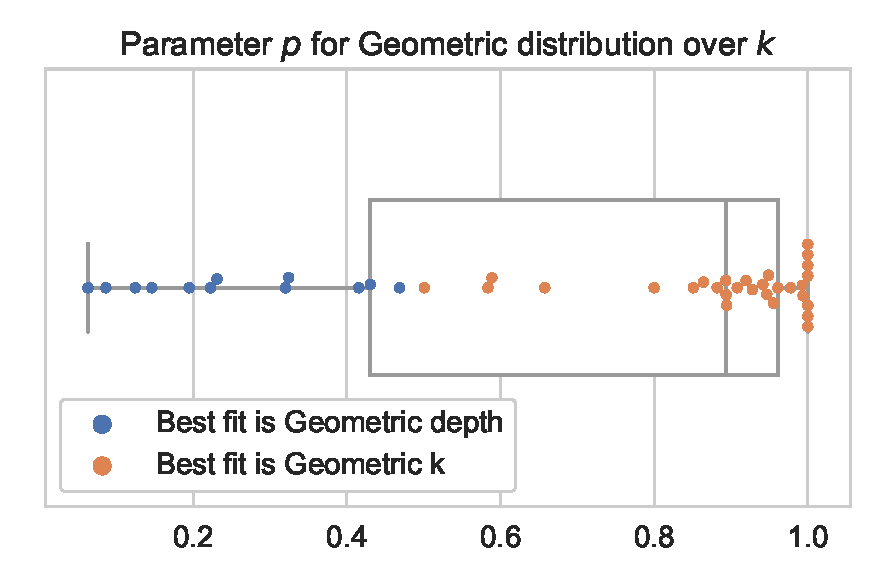
\includegraphics[width=6cm]{geom-k-p}
    \caption{Distribution of parameter $p$ for Geometric distribution over $k$. Each point is the model fit for one participant. The Geometric models over $k$ and $d$ were compared to determine the color of each point.}
\end{figure}


% \section{Experiment 2: Incentives modulating multigoal complexity}
% In Experiment 1, participants were incentivized to find short solutions only to the extent that it allowed them to complete the experiment more quickly. Because executing moves is very fast in this task, the benefit of considering multiple goals (and thus finding shorter solutions) was not great, perhaps outweighed by the cognitive effort associated with more complex multigoals. To explore whether people may adapt the size of their multigoals in response to increasing pressure to solve problems efficiently, we conducted a second experiment in which participants were moetarily incentivized to take as few moves as possible on each problem.

% \section{Methods}
% \subsubsection{Stimuli and procedure}
% The primary modification from Experiment 1 was the introduction of a points system. Participants began each problem with some number of points, which was decremented each time they moved a block. The initial points for each problem was set to the 95\% quantile of the number moves taken on that problem in Experiment 1. After solving each problem, the leftover points were added to a running total. At the end of the experiment, participants were given bonus payments equal to one cent per point. The critical manipulation was to increase the stakes of certain problems, multiplying both the initial point count and the cost-per-move by three. To maximize statistical power, we duplicated each problem from Experiment 1, presenting it once as a low-stakes problem and again as a high-stakes problem. To reduce the probability of participants noticing the duplicates, we swapped the left and right columns of the initial state, a manipulation that changes the visual appearance without altering the abstract structure of the problem. This procedure revealed that two of the problems selected for Experiment 1 were already mirrored duplicates of another problem. We replaced these two problems with new problems, and conservatively set the number of initial points to the largest of the other problems.


% \subsubsection{Participants}
% We recruited 40 participants from Amazon Mechanical Turk. Each participant received \$0.50 for completing the task, plus a performance-dependent bonus (mean: \$3.18). The task took an average of \MISSING minutes.

% \subsection{Results}
% \todo{}

\section{Discussion}
  
To solve complex problems, people have to break them down into smaller problems. The importance of subgoals has been long recognized, and they play a critical role in the most successful models of human problem solving \citep{anderson2013architecture,NewellSimon1972,laird1987soar}. However, these models are limited by the assumption that only one subgoal can be pursued at a time. To address this limitation, we have extended the classic subgoaling model with the notion of a multigoal, a subset of subgoals that is pursued concurrently. Through a formal model comparison, we showed that the multigoal model explains data better than a standard one-at-a-time subgoal model or a model that ignores subgoal structure alltogether.

We have presented a theory of how one might represent and pursue multiple concurrent subgoals, and we have provided preliminary evidence that people actually do this. However, we don't have a theory of how they select which subgoals to pursue at any moment. Thus, in the context of the experiment, we treat $k$ as a latent variable to be inferred, not predicted. A more complete model would explain why people choose the $k$ they do, perhaps as a function of problem complexity or stakes. Such a theory could be constructed within the framework of resource-rational analysis \citep{Griffiths2014}, predicting that people choose a $k$ to optimize a tradeoff between the efficiency of the problem solution and the cost of representing and pursuing more complex multigoals. An important open question is how to quantify the cost of a multigoal, or even a standard subgoal.

Another major direction for future work is to remove the simplifying assumption of subgoal-ordering. This assumption allows us to reduce the problem of composing multigoals from a set of subgoals to the problem of selecting a single integer $k$, greatly simplifying model specification and inference. However many of the problems people are faced with do not have such an assumed ordering. To return to the initial motivating example, you do not know a priori whether you should go to a grocery store or library first. Unfortunately, choosing a multigoal from an unordered set of subgoals is a daunting task. With $n$ basic subgoals, there are $\binom{n}{k}$ possible multigoals of size $k$ that you could construct. But fortunately, as Colton demonstrates when he hands out roses at the end of each episode, people are entirely of capable of choosing $k$ out of $n$ options.

% In the general case with $n$ subgoals, there are $2^n$ possible multigoals. At a practical level, this poses a substantial challenge for infering which multigoal is guiding someone's behavior at any moment. But it also raises a theoretical question: How can people effectively choose multigoals when there are so many options? Addressing this question will be a challenging, but critical direction for future work.




\bibliographystyle{apacite}
\setlength{\bibleftmargin}{.125in}
\setlength{\bibindent}{-\bibleftmargin}

\bibliography{references}


\end{document}
